\documentclass[a4paper]{report} % Changé de 'article' à 'report'

%% Language and font encodings
\usepackage[english, french]{babel}
\usepackage[utf8]{inputenc}
\usepackage[T1]{fontenc}

%% Sets page size and margins
\usepackage{geometry}
\usepackage{lipsum}              % Pour du texte d'exemple (facultatif)

%% Useful packages
\usepackage{amsmath, amssymb}
\usepackage{amssymb} % Redundant if amsmath is used, but kept as in original
\usepackage{graphicx}
\usepackage[colorlinks=true, allcolors=black]{hyperref}
\usepackage{float}
\usepackage{tikz}
\usepackage{calc}
\usepackage{pgfplots}
\usepackage{setspace}
\usepackage{titlesec}
\usepackage{parskip}
\usepackage{tabularx}
\usepackage{booktabs}
\usepackage{enumitem}
\usepackage{xcolor}
\definecolor{accenture}{HTML}{A100FF}
\usetikzlibrary{positioning, shapes.geometric, arrows.meta, shapes.misc, backgrounds, fit, shadows}
\usetikzlibrary{shapes, arrows, positioning}
\setlist[itemize]{itemsep=8pt, topsep=2pt} % Applique ces réglages à toutes les listes itemize
\setcounter{secnumdepth}{3} %pour que le niveau 3 (subsubsection soit numeroté)
\setcounter{tocdepth}{2} %pour que le niveau 2 (subsection apparaisse dans la table des matieres)
% Personnalisation des titres de chapitres
% Met le mot "Chapitre" et son numéro en gras et très grand (\Huge)
% et le titre du chapitre également en \Huge
% Redéfinition complète du format des pages de chapitre


% --- 1. Apparence des titres (police, taille, gras...) ---

\titleformat{\chapter}[display]
  {\normalfont\Huge\bfseries} % Apparence générale : gras et centré
  {\vspace*{50pt}\chaptertitlename\ \thechapter} % Espace au-dessus + Texte "Chapitre X"
  {25pt} % Espace vertical entre "Chapitre X" et le titre du chapitre
  {\Huge} % Taille de la police pour le titre du chapitre

\titleformat{\section}
  {\cleardoublepage\normalfont\LARGE\bfseries} % Police grande et en gras
  {\thesection}
  {1em}
  {}

\titleformat{\subsection}
  {\normalfont\large\bfseries} % Police "large" et en gras
  {\thesubsection}
  {1em}
  {}

\titleformat{\subsubsection}
  {\normalfont\normalsize\bfseries} % Police normale et en gras
  {\thesubsubsection}
  {1em}
  {}


% --- 2. Espacement avant et après les titres ---

% Syntaxe : \titlespacing*{commande}{gauche}{AVANT}{APRES}

\titlespacing*{\section}
  {0pt}      % gauche
  {10ex}      % avant (l'espace que vous vouliez ajouter)
  {3ex}    % après

\titlespacing*{\subsection}
  {0pt}      % gauche
  {6ex}    % avant
  {2.5ex}    % après

\titlespacing*{\subsubsection}
  {0pt}      % gauche
  {4ex}   % avant
  {2.5ex}    % après

\pgfplotsset{compat=1.14}

\setlength{\intextsep}{16pt} % Espace autour des figures dans le texte

%% Added packages for new layout
\usepackage{fancyhdr} % For custom headers and footers

\newcommand\fillin[1]{\makebox[#1]{\dotfill}}


\begin{document}
% La page de garde
\begin{titlepage} % Utiliser l'environnement titlepage pour la page de garde
% Définir une géométrie spécifique pour la page de titre pour éviter le débordement
\newgeometry{inner=1cm, outer=1cm, top=1cm, bottom=0.5cm, includefoot=false, includehead=false}
\pagenumbering{roman} % La numérotation commence ici si désiré pour les pages liminaires
\thispagestyle{empty} % La page de garde ne doit pas avoir d'en-tête/pied de page

% --- START OF FIRST PAGE CONTENT (Logos d'origine rétablis) ---
\begin{tikzpicture}[remember picture, overlay]
% IMPORTANT: Ensure these image files exist in the 'images' subfolder and are valid!
% Logos d'origine de la première page
\node[xshift=-7cm, yshift=-3.1cm] at (current page.north) {
\includegraphics[scale=0.11]{images/logo_ida.png}};
\node[below = 0.5cm] at (current page.north) {
\includegraphics[scale = 0.11]{images/ucbl.jpg}};
\node[xshift=6.8cm, yshift=-3.3cm] at (current page.north) {
\includegraphics[scale=0.11]{images/isfa_logo.jpg}};
\end{tikzpicture}

\vspace*{2.5cm} % Réduction de l'espace vertical

{\Large
{\bfseries
\begin{center}
Mémoire présenté le : \\[0.3cm]
pour l'obtention du Diplôme Universitaire d'actuariat de l'ISFA \\
et l'admission à l'Institut des Actuaires
\end{center}
}
\vspace*{0.5cm} % Réduction de l'espace vertical

\noindent Par : Margot SCHMUTZ \\[0.3cm]
\noindent Titre : Super Mémoire de Margot !
\\[0.3cm]
\noindent Confidentialité : \quad $\boxtimes$ NON \qquad $\square$ (Durée : $\square$ 1 an \quad  $\square$ 2 ans)
\\
\textit{Les signataires s'engagent à respecter la confidentialité indiquée ci-dessus}
\vspace*{0.5cm}

\noindent
\begin{minipage}{0.6\textwidth}
\begin{tabular}{p{7cm}p{4cm}}
\textit{Membres présents du jury de l'Institut des Actuaires} & \textit{Signature} \\[1.2cm]
\fillin{6cm} & \\[0.8cm]
\fillin{6cm} & \\[0.8cm]
\fillin{6cm} & \\[0.8cm]
\textit{Membres présents du jury de l'ISFA} & \\[1.2cm]
\fillin{6cm} & \\[0.8cm]
\fillin{6cm} & \\[0.8cm]
\fillin{6cm} & \\[0.8cm]
\end{tabular}
\rule{0mm}{4.6cm} % Ensure minipage height
\end{minipage}%
\begin{minipage}{0.4\textwidth}
\textit{Entreprise :} \\
\textit{Nom :} \\[0.3cm]
\textit{Signature :} \\[0.5cm]
\textit{Directeur de mémoire en entreprise :} \\
\textit{Nom :}  \\[0.3cm]
\textit{Signature :} \\[0.5cm]
\textit{Invité :} \\
\textit{Nom :} \\[0.3cm]
\textit{Signature :} \\[0.5cm]
\textit{\textbf{Autorisation de publication et de mise en ligne sur un site de diffusion de documents actuariels} (après expiration de l'éventuel délai de confidentialité)}\\[0.2cm]
Signature du responsable entreprise \\
\framebox[7cm]{\rule{0mm}{1.5cm}}
Signature du candidat \\
\framebox[7cm]{\rule{0mm}{1.5cm}}
\end{minipage}
}
% --- END OF FIRST PAGE CONTENT ---
\end{titlepage}
\restoregeometry % Restaurer la géométrie précédente avant de la redéfinir pour le reste du document.

% Redéfinir la géométrie pour le reste du document après la page de garde
\newgeometry{left=2.54cm,right=2.54cm,top=3.54cm,bottom=3.54cm}
\onehalfspacing
% Augmenter headheight pour accommoder des logos plus grands
\setlength{\headheight}{50pt} % Ajusté pour des logos de 1.6cm de hauteur

% Configurer fancyhdr pour les en-têtes et pieds de page personnalisés
\pagestyle{fancy}
\fancyhf{} % Effacer tous les champs d'en-tête et de pied de page

% En-têtes des pages suivantes avec les logos demandés (taille doublée)
% IMPORTANT: Assurez-vous que images/accenture_logo.png existe !
\fancyhead[L]{
\includegraphics[height=1.6cm]{images/accenture_logo.png}} % Logo Accenture à gauche
\fancyhead[R]{
\includegraphics[height=1.6cm]{images/isfa_logo.jpg}}   % Logo ISFA à droite

\fancyfoot[C]{\sffamily \thepage}

\renewcommand{\headrulewidth}{0pt}
\renewcommand{\footrulewidth}{0pt}

% Redéfinir le style 'plain' pour qu'il soit identique à 'fancy' afin que les logos apparaissent sur les premières pages de chapitre (taille doublée)
\fancypagestyle{plain}{%
  \fancyhf{}%
  \fancyhead[L]{
\includegraphics[height=1.6cm]{images/accenture_logo.png}}% Logo Accenture à gauche
  \fancyhead[R]{
\includegraphics[height=1.6cm]{images/isfa_logo.jpg}}%   Logo ISFA à droite
  \fancyfoot[C]{\sffamily \thepage}%
  \renewcommand{\headrulewidth}{0pt}%
  \renewcommand{\footrulewidth}{0pt}%
}


% Contenu principal en une seule colonne
\tableofcontents

% IMPORTANT: Ensure all included .tex files exist in the specified paths
% and do not contain LaTeX errors themselves!
\chapter*{Résumé}
% Ajouter manuellement cette section à la table des matières
\addcontentsline{toc}{chapter}{Résumé}
Petit résumé en français de mon mémoire ?
\chapter*{Abstract}
% Ajouter manuellement cette section à la table des matières
\addcontentsline{toc}{chapter}{Abstract}

It's a brief sum up in english !
\chapter*{Remerciements}
% Ajouter manuellement cette section à la table des matières
\addcontentsline{toc}{chapter}{Remerciements}

Pour la réalisation de ce mémoire, je tiens à adresser mes remerciements à toutes les personnes qui ont contribué de près ou de loin à son élaboration. Que ce soit au travail avec Lionel Aldeberd qui m'a appris énormément, Lucas Blancheton qui a toujours été là pour m'aiguiller dans mes choix. Merci à Luc pour les relectures et à tous mes collègues stagiaires et alternants, Antoine, Cindy, Eleonore, Lucile, Malak, Manon, Nicolas, Tanguy et Titouan pour leur bonne humeur ! J'ai vraiment passé des très chouettes moments à vos côtés !
\chapter*{Synthèse}
% Ajouter manuellement cette section à la table des matières
\addcontentsline{toc}{chapter}{Synthèse}

Un long résumé en français de mon mémoire 
\chapter*{Synthesis}
% Ajouter manuellement cette section à la table des matières
\addcontentsline{toc}{chapter}{Synthesis}

Un long résumé en anglais de mon mémoire


\clearpage
\pagenumbering{arabic}

\chapter*{Introduction}

% Ajouter manuellement cette section à la table des matières
\addcontentsline{toc}{chapter}{Introduction}

Placement privilégié des épargnants français, l'assurance vie a atteint un encours record de 1 989 milliards d'euros à fin 2024 (France Assureurs) \cite{france_assureurs}, confirmant son rôle prépondérant dans le patrimoine financier national. Cette performance est portée par une collecte nette annuelle de +29,4 milliards d'euros, une hausse de 28,2 milliards par rapport à 2023, ce qui témoigne d'une forte attractivité du produit dans un contexte économique incertain. La dynamique de l'année 2024 est marquée par une hausse globale des cotisations de +14 \%, bénéficiant tant aux supports en euros (+17 \%) qu'aux unités de compte (+8 \%). Simultanément, les prestations versées aux assurés sont en recul de 5 \%. Cette combinaison d'une collecte dynamique et de prestations maîtrisées place la gestion actif-passif (ALM) au cœur des enjeux stratégiques pour les assureurs, qui doivent piloter cet afflux de capitaux tout en maintenant l'équilibre entre sécurité et rendement pour les épargnants.

Le secteur de l'assurance vie en France est ainsi confronté à un besoin important de pilotage via la gestion actif-passif (ALM). Pour cela, les assureurs s'appuient sur l'utilisation de modèles ALM. Ces modèles simulent l'impact de différentes stratégies ce qui nécessite cependant un grand nombre de projections stochastiques, cela engendre une contrainte opérationnelle majeure : le temps de calcul. Cette contrainte limite non seulement la capacité à explorer en profondeur l'ensemble des risques et des opportunités, mais freine également l'agilité stratégique et la réactivité des prises de décision. C'est de la rencontre entre ces exigences et des contraintes opérationnelles qu'ont les assureurs qu'est née la problématique de ce mémoire : comment concilier la nécessité de rapidité des calculs avec l'impératif de fidélité des indicateurs de risque ? Ce mémoire se propose d'investiguer cette problématique en étudiant l'impact des techniques d'agrégation du passif, notamment par la création de \textit{model points}, c'est-à-dire une manière simplifiée de représenter les contrats d'assurance. L'enjeu est de déterminer si cette modélisation simplifiée des portefeuilles de contrats peut constituer une approximation fiable pour le pilotage stratégique, et d'évaluer sous quelles conditions une telle simplification est valide sans masquer des dynamiques de risque essentielles au pilotage de l'entreprise.

Pour répondre à cette problématique, ce mémoire adoptera une double approche. Premièrement, il s'agira de développer un générateur de portefeuilles de passif puis le reste de l'analyse portera sur les effets de l'agrégation sur un portefeuille représentatif du marché français. L'objectif est de comprendre comment les risques évoluent à travers une agrégation. Ce mémoire ne se contentera pas d'analyser l'impact d'une seule méthode d'agrégation ; au contraire, plusieurs méthodes et approches seront testées. Le critère de sélection de la méthode la plus pertinente reposera sur un triple objectif : minimiser l'écart des indicateurs clés de Solvabilité II (notamment le Best Estimate et le SCR), optimiser la rapidité des calculs et atteindre le plus haut niveau d'agrégation possible qui garderait une significativité économique pour l'assureur suffisante. L'axe principal de ce mémoire consistera donc à mener une analyse de sensibilités approfondie sur ces portefeuilles, qu'ils soient granulaires ou agrégés. Notre étude s'appuiera sur des indicateurs quantitatifs clés issus de la norme Solvabilité II, en évaluant notamment l'impact des chocs économiques sur le Best Estimate, le Solvency Capital Requirement (SCR) et la Present Value of Future Profits (PVFP). Ces métriques permettront de mesurer rigoureusement comment l'agrégation modifie la perception du risque et la valeur économique du portefeuille.

Ce mémoire s'articulera en un parcours logique et progressif en cinq temps. La première partie posera le cadre conceptuel de l'étude en explorant le contexte réglementaire de Solvabilité II, les produits d'epargne en assurance vie et les fondements des Générateurs de Scénarios Économiques (GSE). Après l'explication du socle théorique, la deuxième partie abordera les principes de la Gestion Actif-Passif (ALM), en détaillant l'architecture du modèle de projection qui servira de base aux travaux de ce mémoire. La troisième partie permettra de poser les bases de l'analyse, avec l'élaboration d'un générateur de portefeuilles de passifs réalistes destiné à produire les données synthétiques cohérentes. Le cœur méthodologique sera présenté en quatrième partie, à travers un protocole d'analyse comparant diverses méthodes d'agrégation afin de choisir celle qui sera utilisée. Enfin, la cinquième partie sera consacrée à l'interprétation des résultats d'agrégations sur des chocs économiques où, par le biais d'analyses de sensibilité approfondies, l'impact de la méthode d'agrégation retenue sur la mesure du risque sera quantifié, validant ainsi la pertinence de l'approche.

\titleformat{\chapter}[display]
  {\normalfont\Huge\bfseries} % Apparence générale : gras et centré
  {\vspace*{50pt}\chaptertitlename\ \thechapter} % Espace au-dessus + Texte "Chapitre X"
  {25pt} % Espace vertical entre "Chapitre X" et le titre du chapitre
  {\Huge} % Taille de la police pour le titre du chapitre
  [\vfill\newpage] % Reste de la page vide et saut de page

\chapter{Cadre théorique et réglementaire du régime Solvabilité II}
\label{chap:contexte}
\newpage
\section{Solvabilité II : principes et objectifs}
\label{sec:spec_av}

\subsection{Historique de la directive européenne}

\subsection{Les trois piliers de S2 : exigences de capital, gouvernance, et transparence}


\section{Définition et calcul du ratio de solvabilité S2}
\label{sec:s2}


\subsection{Une mesure synthétique de la solidité financière d'un assureur}

Définition du ratio S2 : Fonds propres éligibles / SCR

Interprétation économique du ratio (seuil réglementaire de 100 %, zone de confort, zone d’alerte)

Rôle central du ratio dans la communication avec les régulateurs et les investisseurs

\subsection{Le Solvency Capital Requirement (SCR) : estimation des riques extrêmes}

Logique de calcul : capital requis pour absorber un choc extrême avec un niveau de confiance de 99,5 % sur un an

Méthodes de calcul : formule standard vs modèle interne partiel ou complet

Décomposition du SCR : risque de marché, risque de souscription, risque de crédit, risque opérationnel

\subsection{Les fonds propres éligibles : capacité à couvrir les pertes}

Classification des fonds propres : Tier 1, Tier 2, Tier 3

Critères d’éligibilité et ajustements réglementaires

Impact des réévaluations d’actifs, des plus-values latentes et des instruments hybrides

\subsection{Un indicateur sensible aux chocs économiques et aux arbitrages de gestion}

Sensibilité du ratio aux taux d’intérêt, à la volatilité, aux spreads de crédit

Mécanismes de gestion du ratio : couverture du SCR, allocation d’actifs, revalorisation du passif

Enjeux stratégiques : pilotage dynamique de la solvabilité, gestion de la marge de manœuvre

\section{Enjeux de pilotage de la solvabilité}
\label{sec:gse}


\subsection{Rôle de l'anticipation du ratio dans la gestion stratégique}


\subsubsection{Limites opérationnelles des modèles actuels}

\chapter{Super chapitre 2 de Margot !}

% \section{Principes et Enjeux de la Gestion Actif-Passif (ALM)}
% La gestion Actif-Passif (ALM) trouve son origine dans une particularité fondamentale du secteur de l'assurance énoncé précédemment dans le mémoire : le \textbf{cycle de production inversé}. Contrairement à une entreprise classique qui vend un produit avant d'en percevoir le revenu, un assureur collecte des primes aujourd'hui en échange de la promesse de verser des prestations dans un futur lointain et incertain. Ce décalage temporel est au cœur du modèle économique de l'assurance vie.

% Ce mécanisme engendre une inadéquation structurelle (\textit{mismatch}) entre les deux côtés du bilan. D'une part, le passif est constitué d'engagements de longue durée, dont l'échéance et le montant sont soumis à des aléas (mortalité, comportement de rachat des assurés). D'autre part, pour couvrir ces engagements, l'assureur investit les primes sur les marchés financiers, constituant un actif dont la valeur et les flux sont, par nature, volatiles et dépendants du contexte économique.

% Cette inadéquation est renforcée par une interdépendance dynamique et complexe entre l'actif et le passif.

% \begin{itemize}
%     \item \textbf{Le passif influe sur l'actif :} Le versement des prestations (rachats, décès) contraint l'assureur à liquider une partie de ses actifs, parfois dans des conditions de marché défavorables.
%     \item \textbf{L'actif influe sur le passif :} La performance des actifs financiers a un impact direct sur le niveau des engagements. C'est notamment le cas de la \textbf{Participation aux Bénéfices (PB)}, qui dépend des résultats financiers générés par l'assureur. Le Code des assurances impose une redistribution minimale aux assurés, calculée comme suit :
%     \begin{equation}
%         \label{eq:pb_minReg}
%         \text{PB}_{\text{minReg}} = 85\% \times \max(\text{RésFi}, 0) + 
%         \begin{cases}
%             90\% \times \text{RésTech} & \text{si RésTech} \ge 0 \\
%             100\% \times \text{RésTech} & \text{si RésTech} < 0
%         \end{cases}
%     \end{equation}
%     Où le Résultat Financier (RésFi) est directement issu de la performance des actifs et le Résultat Technique (RésTech) des risques de mortalité et de rachat.
% \end{itemize}
% La gestion Actif-Passif est donc la discipline qui vise à piloter les risques nés de cette interdépendance afin d'assurer la solvabilité et d'optimiser la rentabilité de l'acteur.

% \subsection{La Modélisation ALM : un Outil de Projection Essentiel}

% Pour quantifier et piloter les risques complexes découlant de l'inadéquation actif-passif, les assureurs ont recours à des modèles de projection actuariels sophistiqués, communément appelés modèles de Gestion Actif-Passif ou modèles ALM. L'utilité principale de ces modèles est de projeter le bilan d'un assureur, qu'il s'agisse d'un bilan prudentiel sous Solvabilité 2 ou d'un bilan comptable sous les normes IFRS17, afin d'évaluer la santé financière future de l'organisme sur un horizon de long terme. Leur fonctionnement repose sur la combinaison de deux piliers fondamentaux : des scénarios prospectifs sur l'environnement économique et financier, et des hypothèses sur le comportement futur des assurés (lois de mortalité, de rachat, etc.).

% L'approche de modélisation peut être déterministe ou stochastique, chaque approche répondant à des objectifs d'analyse distincts.

% L'approche \textbf{déterministe} consiste à projeter le bilan de l'assureur selon une trajectoire unique et prédéfinie de l'environnement économique. Cette trajectoire, qualifiée de \textbf{scénario central}, est généralement construite à partir de la courbe des taux sans risque fournie par l'EIOPA. Elle permet d'obtenir le (\textit{Best Estimate}) central, c'est à dire la somme des flux futurs actualisés du portefeuille dans un contexte économique considéré comme le plus probable, servant de base pour le plan d'affaires et la valorisation prudentielle.

% Cependant, une approche déterministe ne peut à elle seule capturer l'éventail des risques, notamment ceux liés aux options et garanties financières (par exemple, les Taux Minimum Garantis ou les options de rachat) dont le coût ne se matérialise que dans des conditions de marché adverses. Pour pallier cette limite, une approche \textbf{stochastique} est nécessaire. Celle-ci s'appuie sur un \textbf{Générateur de Scénarios Économiques (GSE)} pour simuler un grand nombre (souvent plusieurs milliers) de trajectoires économiques futures possibles, chacune représentant une évolution plausible des marchés financiers.

% Chaque scénario économique généré sert alors d'input pour une projection complète du modèle ALM. En agrégeant les résultats de ces multiples projections via la \textbf{méthode de Monte Carlo}, l'assureur obtient non plus une seule valeur, mais une distribution des résultats possibles. L'objectif final est de disposer, pour chaque trajectoire, du détail des flux financiers à la maille la plus fine. Cette granularité permet une analyse statistique approfondie des risques, comme le calcul de quantiles (Value at Risk à 99.5\%) pour déterminer le capital de solvabilité requis (SCR) sous Solvabilité 2. Ces modèles stochastiques sont donc au cœur de l'évaluation des risques et de la prise de décision stratégique, et constituent le fondement du modèle de simulation qui sera détaillé dans la suite de ce chapitre.

% \begin{figure}[H]
%     \centering
%     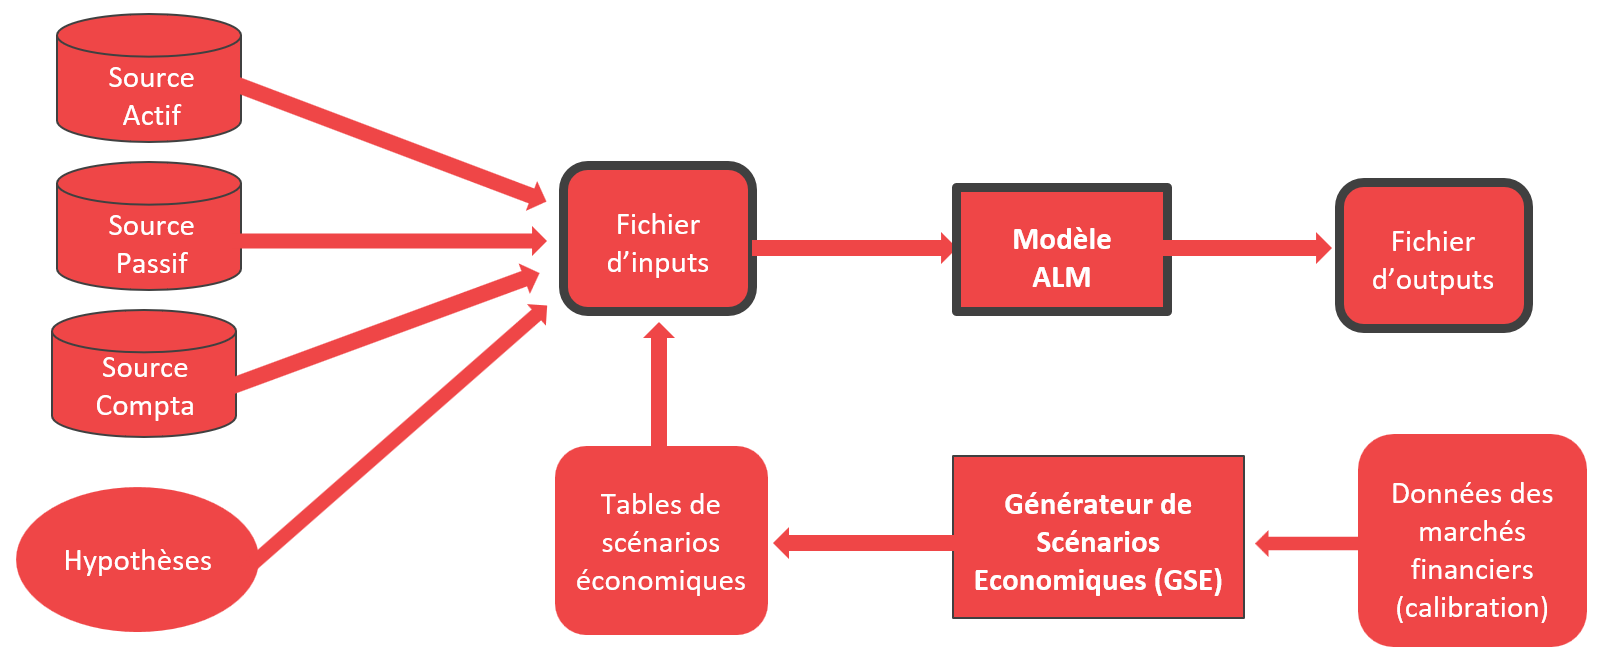
\includegraphics[width=0.8\textwidth]{images/2_chapitres/chapitre2/alm_det.png}
%     \caption{Fonctionnement d'un modèle ALM \textbf{(graphique temporaire)}}
%     \label{fig:alm_det}
% \end{figure}



% \section{Architecture et Fonctionnement du Modèle de Projection}
% \label{sec:architecture_modele}

% L'objectif de cette section est de détailler l'architecture et le séquencement des opérations du modèle ALM développé pour les besoins de cette étude. Le modèle a été conçu pour simuler de manière dynamique et séquentielle le bilan d'un assureur vie sur un horizon de projection pluriannuel.

% Son fonctionnement global peut être décomposé en trois phases principales, comme illustré dans la figure \ref{fig:modele_alm_sequence} :
% \begin{enumerate}
% \item \textbf{Phase d'Initialisation} : Préparation et validation des données d'entrée, et application des chocs réglementaires à la date de départ.
% \item \textbf{Boucle de Projection Annuelle} : Cœur du modèle qui simule, année après année, l'évolution du bilan selon une séquence d'événements prédéfinis.
% \item \textbf{Phase de Finalisation} : Calcul des indicateurs prudentiels et génération des résultats en fin de projection.
% \end{enumerate}

% \begin{figure}[h!]
% \centering
% % Note : Pensez à remplacer le chemin vers votre image
% 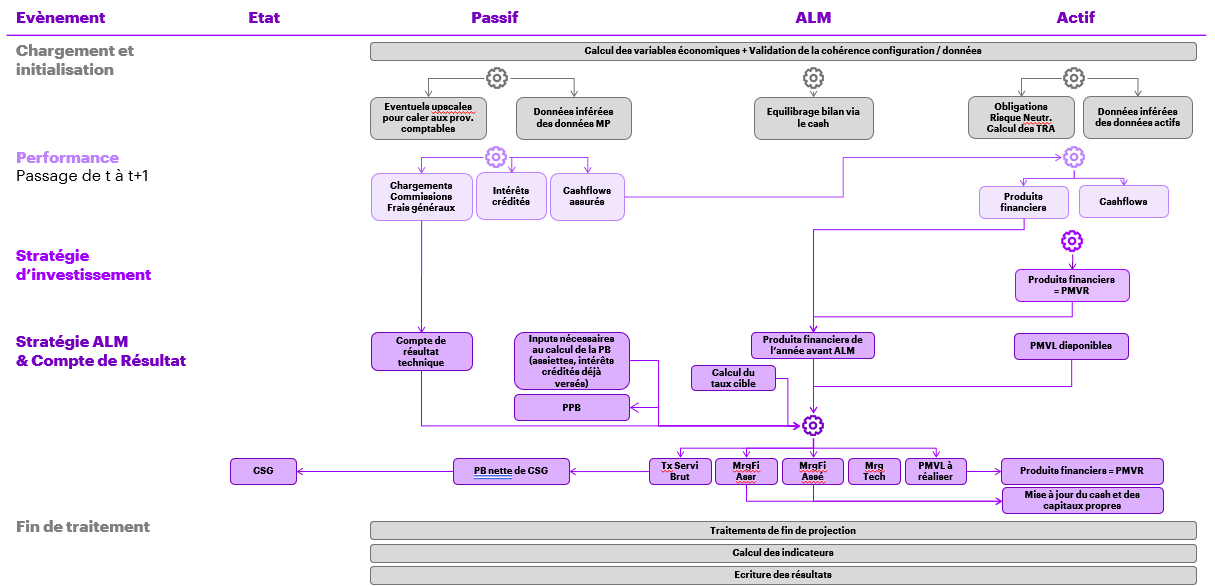
\includegraphics[width=0.98\textwidth]{images/2_chapitres/chapitre2/modele_alm_sequence.png}
% \caption{Architecture générale et séquencement des événements du modèle ALM. \textbf{(graphique temporaire)}}
% \label{fig:modele_alm_sequence}
% \end{figure}

% \subsection{Phase 1 : Initialisation du Modèle}

% Cette première phase prépare l'environnement de projection. Elle est elle-même divisée en trois sous-étapes.

% \subsubsection{Chargement et Validation des Données d'Entrée}

% Le modèle est alimenté par un ensemble de données exhaustif, regroupées en quatre catégories :
% \begin{itemize}
% \item \textbf{Données Économiques et Financières} : Issues du Générateur de Scénarios Économiques (GSE), elles comprennent les courbes de taux, les taux d'inflation et les performances des différentes classes d'actifs pour chaque scénario stochastique.
% \item \textbf{Portefeuille d'Actifs} : Les \textit{model points} d'actifs représentant l'ensemble des placements de l'assureur (obligations à taux fixe et variable, actions et immobilier).
% \item \textbf{Portefeuille de Passifs} : Les \textit{model points} d'épargne décrivant les engagements envers les assurés.
% \item \textbf{Hypothèses de Modélisation} : Un ensemble de tables paramétrant le comportement futur (stratégie d'investissement, stratégie ALM, règles de participation aux bénéfices, tables de mortalité, de rachat) et les chocs prudentiels Solvabilité 2.
% \end{itemize}
% Une étape de validation est systématiquement réalisée pour assurer la cohérence et la qualité des données chargées. Par exemple, nous vérifions qu'il n'y a pas de Provisions mathématiques négatives ou que la somme des taux d'affectation des différentes classes d'actifs est bien égale à 1.

% \subsubsection{Application des Chocs Solvabilité 2 en t=0}

% L'application des chocs instantanés en t=0 est une étape fondamentale du calcul du SCR (Solvency Capital Requirement) selon la formule standard de Solvabilité 2. L'objectif est de mesurer la résilience de l'assureur face à une série de scénarios de crise prédéfinis, calibrés pour représenter un événement se produisant une fois tous les 200 ans.

% Pour chaque choc, le modèle crée un "axe analytique" : les données d'entrée sont dupliquées, puis les paramètres pertinents sont modifiés conformément au scénario de choc. La différence entre la valeur des fonds propres dans le scénario central (sans choc) et leur valeur dans le scénario choqué détermine le besoin en capital pour ce risque spécifique.

% Les principaux chocs, ou modules de risque, se répartissent en plusieurs catégories :

% \begin{itemize} 
%     \item \textbf{Le risque de marché :} Il regroupe les risques liés aux fluctuations des marchés financiers. 
%     \begin{itemize} 
%         \item \textbf{Choc de taux d'intérêt :} Simule une variation soudaine, à la hausse ou à la baisse, de la courbe des taux d'intérêt. Ce choc a un impact majeur sur la valeur des actifs (notamment les obligations) et des passifs (qui sont actualisés avec cette courbe des taux). 
%         \item \textbf{Choc actions :} Modélise une baisse brutale des marchés actions. La formule standard distingue généralement deux types de chocs actions (Type 1 et Type 2) en fonction de la nature et de la diversification des investissements. Par exemple, un choc de -33.84\% pourrait s'appliquer à un portefeuille d'actions diversifié. 
%         \item \textbf{Choc immobilier :} Représente une chute de la valeur du marché immobilier. Le paramètre de -25\% est une valeur standard pour ce type de risque. 
%         \item \textbf{Choc de spread :} Concerne le risque de crédit sur les obligations et les prêts. Il simule un élargissement des spreads de crédit, ce qui diminue la valeur de marché de ces actifs. 
%     \end{itemize}

% \item \textbf{Le risque de souscription vie :} Il est lié aux aléas inhérents à l'activité d'assurance vie.
% \begin{itemize}
% \item \textbf{Choc de mortalité :} Simule une augmentation soudaine et permanente du taux de mortalité (par exemple, +15\%). Ce choc est particulièrement impactant pour les contrats de prévoyance où l'assureur doit verser un capital en cas de décès.
% \item \textbf{Choc de longévité :} À l'inverse, il modélise une baisse permanente du taux de mortalité (les assurés vivent plus longtemps que prévu). Ce risque affecte principalement les rentes viagères, pour lesquelles l'assureur doit verser des prestations plus longtemps.
% \item \textbf{Choc de rachat :} Simule une variation massive et soudaine du comportement des assurés en matière de rachat de leurs contrats. Il se décline en trois sous-modules : une hausse des taux de rachat, une baisse, et un scénario de rachat de masse (catastrophique).
% \item \textbf{Choc de dépenses :} Modélise une augmentation imprévue des frais de gestion de l'assureur, combinée à une hausse de l'inflation de ces frais.
% \item \textbf{Choc de catastrophe :} Concerne les événements extrêmes, comme une pandémie, entraînant une augmentation brutale et temporaire de la mortalité (par exemple, une hausse de 0.15 points de pourcentage du taux de mortalité sur une année).
% \end{itemize}

% \end{itemize}

% \subsubsection{Préparation à la Boucle de Projection}

% Enfin, les tables de données sont préparées pour la projection en y ajoutant les dimensions d'analyse fondamentales : le \textbf{scénario économique}, la \textbf{période de projection} (l'année) et l'\textbf{événement} intra-annuel.

% \subsection{Phase 2 : La Boucle de Projection Annuelle}

% Le cœur du modèle est une boucle itérative qui projette le bilan année par année. Pour chaque pas de temps, trois événements clés sont modélisés séquentiellement.

% \subsubsection{Événement 1 : Performance}
% Cette première étape simule le "passage du temps" sans intervention active du management.
% \begin{itemize}
% \item \textbf{Côté Passif} : Les engagements évoluent sous l'effet des flux biométriques (décès), comportementaux (rachats), et contractuels (arrérages de rente). La provision mathématique est revalorisée en appliquant les Taux Minimums Garantis (TMG) pour les fonds euros et la performance des marchés pour les Unités de Compte (UC).
% \item \textbf{Côté Actif} : La valeur des actifs est mise à jour pour refléter la performance des marchés. Les revenus (coupons, dividendes) sont encaissés et alimentent la trésorerie.
% \end{itemize}

% \subsubsection{Événement 2 : Stratégie d'Investissement}
% Cette étape modélise les décisions de gestion financière. L'algorithme simule la politique d'investissement en cherchant à maintenir une allocation d'actifs cible. En fonction de la trésorerie disponible, le modèle arbitre entre les différentes classes d'actifs, générant des ordres d'achats et de ventes.

% \subsubsection{Événement 3 : Stratégie ALM et Clôture du Compte de Résultat}
% C'est l'étape finale de l'exercice annuel, qui vise à équilibrer le bilan.
% \begin{enumerate}
% \item \textbf{Détermination du Résultat Financier} : Le modèle agrège l'ensemble des produits financiers générés.
% \item \textbf{Application de la Stratégie de Participation aux Bénéfices (PB)} : Le modèle calcule la PB à distribuer, en respectant les contraintes réglementaires et en visant un taux cible. Il peut activer des leviers comme la reprise de la Provision pour Participation aux Excédents (PPE) ou la réalisation de plus-values latentes.
% \item \textbf{Clôture des Comptes} : Le résultat technique et financier sont finalisés pour établir le compte de résultat et s'assurer de l'équilibre du bilan de clôture.
% \end{enumerate}

% \subsection{Phase 3 : Finalisation et Génération des Outputs}

% Une fois la boucle achevée pour toutes les années et tous les scénarios, le modèle entre dans sa phase finale.

% \subsubsection{Calcul des Indicateurs Prudentiels}
% Le principal objectif est de calculer le \textbf{Best Estimate (BE)} des passifs. Pour chaque scénario, le modèle agrège les flux de passifs futurs et les actualise en utilisant les courbes de taux sans risque correspondantes. La moyenne des BE sur l'ensemble des scénarios fournit la valeur centrale, tandis que la distribution permet de calculer le capital de solvabilité requis (SCR).

% \subsubsection{Génération des Rapports de Sortie}
% Enfin, le modèle produit un ensemble de rapports détaillés (similaires aux QRTs réglementaires) présentant les bilans projetés, les comptes de résultat, la décomposition du BE et du SCR, et d'autres indicateurs clés pour l'analyse actuarielle.

% \section{Limites Actuelles du modèle}
% A date, les fonds propres ne sont pas modélisés dans le modèle ALM. En effet, le modèle se concentre sur la projection de l'actif et du passif, ainsi que sur les interactions entre les deux, mais n'intègre pas encore la dynamique des fonds propres. Cette limitation est importante car les fonds propres jouent un rôle crucial dans la solvabilité et la résilience financière de l'assureur. Leur modélisation permettrait de mieux évaluer l'impact des stratégies de gestion sur la solidité financière globale de l'entreprise. L'absence des fonds propres nous empêche de calculer des indicateurs cruciaux tels que le ratio de solvabilité.

% % \chapter{La Gestion Actif-Passif et développement d'un modèle ALM en Python}
% % \section{La gestion Actif-Passif (ALM) : définitions et enjeux}
% % \label{sec:alm}

% % \subsection{Le cycle de production inversé, origine de l'inadéquation Actif-Passif}

% % La gestion Actif-Passif (ALM) trouve son origine dans une particularité fondamentale du secteur de l'assurance que l'on a énoncé dans le début de ce chapitre : le \textbf{cycle de production inversé}. Contrairement à une entreprise classique qui vend un produit avant d'en percevoir le revenu, un assureur collecte des primes aujourd'hui en échange de la promesse de verser des prestations dans un futur lointain et incertain. Ce décalage temporel est au cœur du modèle économique de l'assurance vie.

% % Ce mécanisme engendre une inadéquation structurelle (\textit{mismatch}) entre les deux côtés du bilan. D'une part, le passif est constitué d'engagements de longue durée, dont l'échéance et le montant sont soumis à des aléas (mortalité, comportement de rachat des assurés). D'autre part, pour couvrir ces engagements, l'assureur investit les primes sur les marchés financiers, constituant un actif dont la valeur et les flux sont, par nature, volatiles et dépendants du contexte économique.

% % Cette inadéquation est renforcée par une interdépendance dynamique et complexe entre l'actif et le passif.

% % \begin{itemize}
% %     \item \textbf{Le passif influe sur l'actif :} Le versement des prestations (rachats, décès) contraint l'assureur à liquider une partie de ses actifs, parfois dans des conditions de marché défavorables.
% %         \item \textbf{L'actif influe sur le passif :} La performance des actifs financiers a un impact direct sur le niveau des engagements. C'est notamment le cas de la \textbf{Participation aux Bénéfices (PB)}, qui dépend des résultats financiers générés par l'assureur. Le Code des assurances impose une redistribution minimale aux assurés, calculée comme suit :
% %         \begin{equation}
% %             \label{eq:pb_minReg}
% %             \text{PB}_{\text{minReg}} = 85\% \times \max(\text{RésFi}, 0) + 
% %             \begin{cases}
% %                 90\% \times \text{RésTech} & \text{si RésTech} \ge 0 \\
% %                 100\% \times \text{RésTech} & \text{si RésTech} < 0
% %             \end{cases}
% %         \end{equation}
% %         Où le Résultat Financier (RésFi) est directement issu de la performance des actifs et le Résultat Technique (RésTech) des risques de mortalité et de rachat.
% % \end{itemize}
% % La gestion Actif-Passif est donc la discipline qui vise à piloter les risques nés de cette interdépendance afin d'assurer la solvabilité et d'optimiser la rentabilité de l'acteur.

% % \subsection{Objectifs et périmètre de l'ALM}

% % % À COMPLÉTER :
% % % Expliquer ici les trois grands objectifs de l'ALM :
% % % 1. Maîtriser les risques (taux, marché, liquidité...).
% % % 2. Assurer la solvabilité réglementaire (respect du SCR).
% % % 3. Optimiser la rentabilité (maximiser le rendement pour un risque donné).


% % \subsection{Le modèle ALM : un outil de simulation prospective}

% % % À COMPLÉTER :
% % % Décrire ici le rôle du modèle ALM comme outil de prise de décision.
% % % - Principe : simulation conjointe de l'actif et du passif sur le long terme.
% % % - Inputs principaux : GSE, lois de comportement, portefeuille, règles de gestion.
% % % - Mentionner que vous utilisez un tel outil dans le cadre de votre mémoire, sans pour autant faire une étude ALM complète.


% % \subsection{Principaux indicateurs de pilotage ALM}

% % % À COMPLÉTER :
% % % Lister et décrire brièvement quelques indicateurs clés issus des modèles ALM.
% % % - Projection de la NAV (fonds propres prudentiels).
% % % - Évolution du ratio de couverture SCR.
% % % - Analyses de sensibilité et stress tests (impact d'un choc de taux, actions, etc.).

% % La réalisation des analyses de sensibilités, cœur de ce mémoire, s'appuie sur un moteur de projection robuste : le modèle ALM (Asset Liability Management). Historiquement, le modèle utilisé au sein d'forsides reposait sur une architecture en VBA (Visual Basic for Applications). Pour des impératifs de performance, de maintenabilité et de flexibilité, la décision a été prise de développer un nouveau modèle en Python. Cette migration a été l'occasion de repenser l'architecture du modèle pour mieux répondre aux exigences de calcul complexes de Solvabilité 2.

% % Ce chapitre décrit ce nouveau modèle ALM. Nous présenterons son architecture globale, son fonctionnement détaillé à travers la projection des actifs, des passifs et la mise en œuvre des stratégies de gestion, et nous conclurons sur ses limites actuelles qui ouvrent des perspectives d'amélioration.

% % \section{Développement du Modèle ALM en Python}

% % La transition d'un modèle ALM de VBA vers Python a été motivée par la recherche de performance, de maintenabilité et de modularité. Le langage Python, avec son écosystème de librairies scientifiques comme \textit{NumPy}, \textit{Pandas} ou \textit{Polars}, offre un cadre de développement beaucoup plus robuste et performant pour des calculs actuariels intensifs.

% % \subsection{Présentation du modèle ALM développé pour forsides}

% % Le modèle ALM a pour objectif principal de projeter l'ensemble des actifs et des passifs d'un assureur sur un horizon de long terme (typiquement 40 à 60 ans), sous un grand nombre de scénarios économiques stochastiques. Ces projections permettent de calculer les indicateurs prudentiels requis par la directive Solvabilité 2, notamment le BE et le SCR. Le modèle se veut un outil de pilotage stratégique, capable de simuler l'impact de différentes stratégies de gestion d'actifs, de politiques de souscription ou de participation aux bénéfices.

% % \subsection{Fonctionnement du modèle ALM}

% % \subsubsection{Fonctionnement général du modèle}
% % Le modèle opère de manière itérative, année par année, pour chaque scénario économique. À chaque pas de temps, il simule l'ensemble des flux financiers et des opérations de bilan. Le processus global peut être résumé comme suit :
% % \begin{enumerate}
% % \item \textbf{Entrées :} Le modèle prend en entrée le portefeuille de passifs (issu du générateur ou d'un client), le portefeuille d'actifs, un set de scénarios économiques (ESG), et les règles de gestion (stratégie d'investissement, politique de PB, etc.).
% % \item \textbf{Moteur de projection :} Pour chaque année et chaque scénario, le moteur calcule les flux de passifs, les flux d'actifs, et applique les décisions de gestion.
% % \item \textbf{Sorties :} En fin de projection, le modèle génère des comptes de résultat et des bilans prévisionnels pour chaque scénario, qui sont ensuite utilisés pour calculer les indicateurs S2 par agrégation et analyse statistique.
% % \end{enumerate}

% % \subsubsection{Fonctionnement du passif}
% % La projection du passif consiste à simuler l'évolution du portefeuille de contrats. À chaque pas de temps, le modèle calcule :
% % \begin{itemize}
% % \item Les primes encaissées.
% % \item Les prestations versées (décès, rachats, rentes).
% % \item Les chargements et frais prélevés.
% % \item L'évolution des provisions mathématiques, en tenant compte de la revalorisation issue de la participation aux bénéfices.
% % \end{itemize}
% % Les flux de prestations sont déterminés par l'application des lois de comportement (mortalité, rachat) sur le portefeuille des assurés survivants.

% % \subsubsection{Fonctionnement de l'actif}
% % Simultanément, le modèle projette la valeur du portefeuille d'actifs. Pour chaque classe d'actifs (actions, obligations, immobilier, etc.), il calcule :
% % \begin{itemize}
% % \item L'évolution de la valeur de marché, en fonction des indices fournis par le scénario économique.
% % \item Les revenus générés (dividendes, coupons, loyers).
% % \end{itemize}
% % Le modèle gère également le réinvestissement des flux de trésorerie et les opérations d'achat/vente décidées par la stratégie d'investissement.

% % \subsubsection{Fonctionnement de la stratégie d'investissement}
% % La stratégie d'investissement est un ensemble de règles qui dictent la manière dont l'actif est géré. Le modèle implémente une allocation stratégique cible (\textit{Strategic Asset Allocation} - SAA). Chaque année, il compare l'allocation réelle du portefeuille à l'allocation cible et déclenche des opérations d'achat ou de vente pour réduire l'écart, dans le respect des contraintes de liquidité et de transaction.

% % \subsubsection{Fonctionnement de la stratégie ALM et de la politique de PB}
% % Le cœur du modèle ALM est l'interaction entre l'actif et le passif. Le résultat financier généré par l'actif est utilisé pour déterminer la revalorisation servie aux assurés. La politique de Participation aux Bénéfices (PB) est une fonction clé qui répartit la performance financière entre l'assureur et les assurés, dans le respect des engagements contractuels et réglementaires. Le modèle simule la constitution et la reprise de la Provision pour Participation aux Bénéfices (PPB), qui permet de lisser les taux servis dans le temps.

% % \subsection{Limites actuelles du modèle}
% % Malgré sa robustesse, le modèle actuel présente certaines limites. Les règles de gestion, notamment la stratégie d'investissement, sont encore modélisées de manière relativement statique et ne réagissent pas toujours de façon dynamique aux conditions de marché extrêmes. De plus, la granularité de certains modules pourrait être affinée, notamment en ce qui concerne la modélisation des frais ou des impôts. Enfin, bien que les performances aient été grandement améliorées par rapport à la version VBA, les temps de calcul pour des portefeuilles très volumineux sur des milliers de scénarios restent un défi et une piste d'optimisation continue.
\chapter{Construction d'un Générateur de Portefeuilles de Passifs Réaliste}

\section{Objectifs Stratégiques et Contraintes Techniques}
La capacité à tester la robustesse des modèles et la pertinence des analyses de sensibilité repose sur un prérequis fondamental : la disponibilité de données de passif variées et réalistes. Pour un cabinet de conseil, où l'accès aux portefeuilles des clients n'est pas systématique, la faculté de générer des portefeuilles synthétiques, mais représentatifs du marché, constitue un atout stratégique majeur. C'est dans ce contexte qu'un générateur de portefeuilles de passifs a été conçu et développé dans le cadre de ce mémoire.

Ce chapitre a pour vocation de présenter cet outil essentiel. Nous détaillerons les besoins stratégiques et analytiques auxquels il répond, la méthodologie de génération retenue, les contraintes techniques rencontrées et les données qui ont été utilisées pour rendre le portefeuille le plus réaliste possible.

Pour l'instant ce chapitre n'est pas encore terminé, le générateur de portefeuilles de passifs n'étant pas encore finalisé, voici une partie temporaire le présentant avec des remarques réalisées dans le but d'améliorer le générateur ainsi que la qualité de ce chapitre dans le mémoire. C'est un chapitre crucial car c'est ici que seront introduites les données sur lesquelles les analyses seront basées.
 
\subsection{Définition du générateur de portefeuilles de passifs}
Un générateur de portefeuille de passifs est un outil logiciel conçu pour créer, de manière algorithmique, des ensembles de données synthétiques qui imitent avec réalisme des portefeuilles de contrats d'assurance-vie. Plutôt que de s'appuyer sur des données réelles, souvent confidentielles ou indisponibles, cet outil simule les caractéristiques fondamentales des assurés (âge, sexe, etc.) et de leurs contrats (type de produit, montant de la provision mathématique, date de souscription, etc.).

L'objectif n'est pas de produire des données aléatoires, mais de générer un portefeuille dont les propriétés statistiques — distributions, corrélations, tendances — sont indiscernables de celles d'un portefeuille réel. Il s'agit d'une brique essentielle pour l'analyse quantitative en actuariat, permettant de surmonter les contraintes d'accès aux données. Le développement d'un tel outil s'est imposé comme une nécessité pour plusieurs raisons stratégiques et analytiques, tant pour un cabinet de conseil, qui peut ainsi tester ses modèles sans données client, que pour un organisme d'assurance souhaitant explorer des scénarios prospectifs et évaluer l'impact de nouvelles offres.


\subsection{Besoins métiers : simulation de nouveaux produits et analyse concurrentielle}

Pour un acteur du secteur de l'assurance, qu'il s'agisse d'un assureur ou d'un cabinet de conseil, la capacité à modéliser et à anticiper les dynamiques de marché est un avantage concurrentiel décisif. Le générateur de portefeuilles de passifs répond directement à ce besoin en fournissant un support quantitatif pour la prise de décision stratégique, notamment dans trois domaines clés : le lancement de nouveaux produits, l'orientation du \textit{business mix} et l'analyse concurrentielle.

Premièrement, le lancement d'un nouveau produit d'assurance-vie représente un investissement et un risque significatifs. Avant toute commercialisation, il est impératif d'en évaluer rigoureusement les impacts sur le profil de risque et la rentabilité de l'entreprise. Le générateur offre un véritable laboratoire virtuel pour ce faire. En simulant l'intégration de milliers de polices conformes aux caractéristiques du nouveau produit (garanties, frais, options), il permet de projeter leur comportement dans le temps. Il devient alors possible d'analyser leur effet sur les indicateurs prudentiels de Solvabilité II, tels que le \textit{Best Estimate} (BE) et le besoin en capital (\textit{Solvency Capital Requirement} - SCR), mais aussi d'évaluer leur sensibilité à divers chocs de marché (hausse des taux, krach boursier) ou de comportement (vagues de rachats). Cet outil permet ainsi de tester, d'ajuster et d'optimiser les caractéristiques d'un produit pour atteindre le couple rendement/risque désiré avant même sa mise sur le marché.

Deuxièmement, le générateur est un outil précieux pour piloter la stratégie à long terme de l'entreprise. La direction peut être amenée à vouloir faire évoluer son \textit{business mix}, c'est-à-dire la répartition de son portefeuille entre différents types de produits (fonds en euros, unités de compte, prévoyance...). Par exemple, dans un contexte de taux bas persistants, un assureur pourrait vouloir accélérer sa transition vers les produits en unités de compte. Le générateur permet de quantifier les implications d'une telle stratégie. En simulant des portefeuilles futurs correspondant à ces nouvelles orientations commerciales, la direction peut visualiser les conséquences sur le bilan, la rentabilité prévisionnelle, mais aussi sur la consommation de capital et l'exposition aux risques. Ces simulations éclairent les décisions stratégiques et s'intègrent naturellement dans des exercices prospectifs comme l'ORSA (\textit{Own Risk and Solvency Assessment}).

Enfin, la capacité à se positionner par rapport à ses concurrents est fondamentale. Faute d'accès aux portefeuilles détaillés des autres acteurs, un assureur doit s'appuyer sur des reconstitutions. En se basant sur des données publiques (rapports annuels, publications réglementaires comme les SFCR) ou des statistiques sectorielles, le générateur peut créer un portefeuille "moyen" représentatif du marché, ou simuler le portefeuille probable d'un concurrent spécifique. Ces portefeuilles synthétiques deviennent alors une base solide pour des analyses comparatives (\textit{benchmarking}). Ils permettent non seulement d'évaluer la performance relative, mais aussi de comparer les profils de risque, d'anticiper les stratégies concurrentes et d'identifier les meilleures pratiques du marché. Il convient toutefois de souligner les limites d'une telle démarche. Une analyse ALM complète et réaliste d'un concurrent ne peut se contenter de la seule modélisation du passif. Elle exigerait également de simuler son portefeuille d'actifs et de disposer d'informations précises sur ses ressources financières et ses fonds propres. Or, ces données, qui relèvent du secret des affaires, sont rarement publiques. Par conséquent, l'analyse comparative reste nécessairement partielle, se concentrant sur les caractéristiques intrinsèques du portefeuille de passifs reconstitué.
\bigskip

\begin{figure}[h!]
    \centering
    \begin{tikzpicture}[
        node distance=1ex,
        box/.style={
            rectangle,
            rounded corners=4pt,
            draw=gray,
            fill=white,
            very thin,
            inner sep=15pt,
            minimum width=3cm,
            minimum height=2cm,
            align=center,
            font=\sffamily\bfseries\color{black}
        },
        arrow/.style={
            -Latex,
            very thin,
            color=accenture,
            line width=2pt
        }
    ]

    % Nodes
    \node[box] (input) {Données d'entrée :\\- Rapports d'assureurs\\- Marché français};
    \node[box, right=4ex of input] (process) {Modélisation et calibrage :\\- Distributions\\- Corrélations};
    \node[box, right=4ex of process] (output) {Portefeuille synthétique};

    % Arrows
    \draw [arrow] (input) -- (process);
    \draw [arrow] (process) -- (output);

    \end{tikzpicture}
    \caption{Schéma de la méthodologie de génération d'un portefeuille de passifs synthétique.}
    \label{fig:methodologie_horizontale}
\end{figure}

\subsection{Défis de la modélisation : réalisme, volumétrie et flexibilité}

La conception et la mise en œuvre d'un générateur de portefeuilles de passifs efficace soulèvent trois défis majeurs et interdépendants : le réalisme des données générées, la gestion de la volumétrie et la flexibilité de l'outil.

Le premier défi, et le plus fondamental, est celui du réalisme. Il ne s'agit pas de produire des données aléatoires, mais de créer un portefeuille synthétique dont les propriétés statistiques sont indiscernables de celles d'un portefeuille réel. Cela implique non seulement de reproduire fidèlement les distributions de chaque caractéristique individuelle (âge, montant, etc.), mais aussi, et surtout, de capturer les corrélations complexes qui les lient. Par exemple, l'âge d'un assuré est souvent corrélé au type de produit souscrit et au montant de sa provision mathématique. Ignorer ces dépendances conduirait à un portefeuille incohérent, dont le comportement sous différents scénarios de risque serait erroné, invalidant ainsi les analyses prudentielles ou stratégiques qui en découlent.

Le deuxième défi est celui de la volumétrie. Les portefeuilles d'assurance-vie des grands acteurs du marché se comptent en centaines de milliers, voire en millions de contrats. Le générateur doit être capable de produire des ensembles de données de cette ampleur de manière performante, c'est-à-dire dans un temps de calcul raisonnable et sans consommer une quantité prohibitive de ressources mémoire. Cette contrainte de performance est d'autant plus forte que la gestion des corrélations, nécessaire au réalisme du portefeuille, ajoute une complexité de calcul significative. En effet, la modélisation des dépendances entre variables (par exemple, via des méthodes comme les copules) est intrinsèquement plus coûteuse en ressources que la simple génération de variables indépendantes. Il faut donc trouver un équilibre entre la sophistication statistique et la performance, ce qui a des implications directes sur les choix technologiques et algorithmiques, écartant les solutions naïves au profit d'approches optimisées pour le traitement de données massives.

Enfin, le troisième défi est la flexibilité. Un générateur ne serait que d'une utilité limitée s'il ne produisait qu'un seul type de portefeuille statique. Pour répondre aux besoins métiers variés, l'outil doit être hautement paramétrable. L'utilisateur doit pouvoir ajuster finement les caractéristiques du portefeuille à générer : définir les spécificités d'un nouveau produit, modifier les distributions statistiques pour simuler un segment de marché différent, ou encore changer les lois de comportement (rachat, mortalité) pour tester de nouvelles hypothèses. Cette flexibilité est la clé qui transforme le générateur en un véritable laboratoire d'expérimentation pour les actuaires et les stratèges.


\section{Méthodologie de Génération et Modélisation Statistique}

La méthodologie de génération du portefeuille de passifs synthétique est au cœur de notre démarche. Elle vise à construire un ensemble de contrats d'assurance dont les propriétés statistiques sont entièrement maîtrisées, en s'appuyant sur une approche stochastique. Le principe fondamental consiste à modéliser chaque caractéristique d'un contrat (âge de l'assuré, montant de la provision, etc.) comme une variable aléatoire tirée d'une loi de probabilité calibrée sur des données de marché.


\subsection{Approche stochastique par lois de probabilité}

Le cœur du générateur de passifs repose sur la modélisation de chaque attribut d'un contrat d'assurance vie par une loi de probabilité spécifique. Ce processus permet de créer une population de polices hétérogène et réaliste, dont la diversité est essentielle pour une simulation ALM pertinente. La génération s'effectue en deux temps : d'abord, la définition de "produits types" ou archétypes, puis la génération des contrats individuels à partir de ces archétypes. \textit{Note pour moi-même : Le concept d'archétypes est une bonne idée, mais je dois le rendre plus concret. Je devrais définir précisément ce que c'est, combien j'en ai créé et sur quelle base (ex: "fonds en euros sécuritaire", "mixte dynamique", "pur UC"). Un tableau récapitulatif des archétypes et de leurs caractéristiques serait une excellente addition pour clarifier ce point.}

Les caractéristiques de ces profils (par exemple, les fourchettes de Taux Minimum Garanti (TMG), les montants moyens de provision mathématique) sont elles-mêmes générées aléatoirement à l'aide de lois uniformes, discrètes ou continues. Cette première étape permet de fixer les méta-paramètres (tels que la moyenne $\mu$, l'écart-type $\sigma$, ou les bornes $[min, max]$) qui régiront la génération fine des contrats. \textit{Note pour moi-même : Attention, ce passage est confus. Est-ce que je tire les paramètres des archétypes aléatoirement ? Si c'est le cas, je dois justifier cette couche de stochasticité. Sinon, si les paramètres sont fixés par des hypothèses expertes, je dois le dire clairement. Je devrais reformuler en précisant que "Les paramètres définissant chaque archétype (fourchettes de TMG, etc.) sont déterminés en amont..." pour plus de clarté.}

Chaque contrat individuel est ensuite instancié en tirant ses variables selon des lois de probabilité spécifiques, reflétant la nature de la caractéristique modélisée :
\begin{itemize}
    \item \textbf{Nombre de polices par agrégat :} Modélisé par une loi de Poisson $\mathcal{P}(\lambda)$, tronquée pour assurer une valeur minimale de 1. \textit{Note pour moi-même : Je dois justifier le choix de la loi de Poisson. C'est un choix classique, mais je dois expliquer pourquoi je l'ai fait (ex: grand nombre de clients potentiels, faible probabilité de souscription). Je dois aussi préciser comment le paramètre lambda est calibré. Pour la "troncature à 1", je dois être plus précis mathématiquement. Est-ce que j'utilise une loi de Poisson tronquée en zéro (Zero-Truncated Poisson) ? Si oui, je devrais donner la fonction de masse correspondante.}
    \item \textbf{Sexe de l'assuré :} Modélisé par une loi de Bernoulli $\mathcal{B}(p)$, où $p$ représente la proportion d'hommes définie dans les spécifications du produit. \textit{Note pour moi-même : C'est un choix standard. Je dois juste préciser d'où vient le paramètre p. Est-ce que je l'ai tiré des données de marché, des statistiques nationales (INSEE), ou est-ce une hypothèse propre au produit cible ?}
    \item \textbf{Montants des provisions (fonds euros et UC) :} Tirés selon une loi Normale $\mathcal{N}(\mu, \sigma^2)$, dont les paramètres sont issus des spécifications. Les valeurs générées sont ensuite tronquées pour rester dans des bornes prédéfinies, afin d'éviter les valeurs aberrantes. \textit{Note pour moi-même : Le choix de la loi Normale pour des montants est discutable. Une loi Lognormale ou Gamma serait peut-être plus adaptée. Je dois justifier ce choix. Ai-je fait des tests d'ajustement (Kolmogorov-Smirnov, etc.) sur des données réelles ? Je dois aussi détailler la troncature : quelles bornes [min,max] et comment ont-elles été choisies ? Je dois vérifier si j'ai bien tenu compte de l'impact de la troncature sur la moyenne et la variance pour que les moments finaux correspondent aux cibles.}
    \item \textbf{Allocation d'actifs cible :} Les poids cibles pour chaque classe d'actifs (actions, immobilier, etc.) sont également générés suivant des lois Normales. Un mécanisme de normalisation est ensuite appliqué pour garantir que la somme des allocations $\sum_{i} \omega_i$ pour un contrat donné est égale à 1. \textit{Note pour moi-même : Même remarque que pour les provisions. La normalisation post-tirage modifie les lois marginales. Une approche plus rigoureuse serait d'utiliser une loi de Dirichlet. Je devrais mentionner cette alternative et justifier pourquoi je ne l'ai pas utilisée (par exemple, pour des raisons de simplicité).}
    \item \textbf{Date d'effet du contrat :} Générée par une loi Uniforme continue sur un intervalle de temps $[T_{\text{début}}, T_{\text{fin}}]$. \textit{Note pour moi-même : C'est un choix simple. Je dois le justifier brièvement. Est-ce que l'hypothèse d'une souscription uniforme dans le temps est réaliste pour mon cas ? Je pourrais mentionner que d'autres lois comme Beta ou Triangulaire pourraient mieux modéliser des pics de souscription.}
\end{itemize}

\subsection{Calibration des distributions marginales à partir des données de marché}

L'approche stochastique adoptée n'est pas purement aléatoire ; elle est rigoureusement calibrée pour refléter une réalité de marché ou un portefeuille cible. La calibration des distributions marginales de chaque variable est assurée principalement via un ensemble de spécifications qui définissent les paramètres des lois de probabilité. Ces spécifications peuvent être obtenues de deux manières complémentaires :
\begin{enumerate}
    \item \textbf{Calibration par hypothèses expertes :} Les paramètres des lois (moyennes, écarts-types, bornes) sont définis sur la base d'hypothèses actuarielles et économiques. Cette méthode est utilisée pour explorer des scénarios de marché spécifiques ou pour concevoir des produits cibles. \textit{Note pour moi-même : Ce paragraphe est trop vague, il faut que je le rende plus concret avec des exemples précis.}
    \item \textbf{Calibration directe sur données réelles :} Les spécifications peuvent être issues d'une analyse statistique d'un portefeuille existant. Les paramètres des lois sont alors les estimateurs directs des moments empiriques (moyenne, variance) observés sur les données, garantissant que le portefeuille synthétique réplique fidèlement la structure du portefeuille réel. \textit{Note pour moi-même : C'est le point le plus faible de la section, je dois absolument le renforcer. Je dois décrire précisément la source de données utilisée (portefeuille réel anonymisé ? taille ? période ?). Je dois expliquer la méthode d'estimation (méthode des moments ou maximum de vraisemblance ? Pourquoi ce choix ?). Surtout, je dois ajouter la validation statistique : quels tests d'ajustement (goodness-of-fit) ai-je utilisés (Chi-deux, K-S) et quels sont les résultats (p-valeurs) ? Des graphiques comparant l'histogramme des données réelles et la densité de la loi calibrée sont indispensables ici.}
\end{enumerate}

Un exemple particulièrement abouti de cette calibration est la modélisation de la distribution des âges des assurés. Le processus charge une distribution d'âge de référence, représentative de la population cible. Cette distribution est ensuite transformée en une série de lois de probabilité conditionnelles : pour chaque âge maximum possible à la souscription, $n$, une distribution de probabilité discrète, tronquée à $n$, est calculée. \textit{Note pour moi-même : C'est un bon exemple, mais je dois être plus précis. Quelle est la "distribution d'âge de référence" ? Table de mortalité réglementaire, données INSEE ? Je dois citer la source exacte. Je devrais aussi décrire le processus mathématiquement. Si $f(x)$ est la densité de référence, la densité conditionnelle est $f_{X \mid X \leq n}(x) = \frac{f(x)}{\int_0^n f(t)dt}$. Montrer cette formule prouverait ma maîtrise du sujet.}
Lors de la génération, l'âge d'un assuré pour un contrat donné est tiré au hasard en utilisant la distribution de probabilité conditionnelle qui respecte l'âge maximum autorisé pour ce produit. Cette méthode garantit que la structure démographique du portefeuille généré est cohérente avec celle de la population de référence.

\subsection{Perspective : modélisation des dépendances par la théorie des copules}

\textit{Note pour moi-même : Cette partie devrait plutôt aller dans une conclusion pour donner une ouverture à mon sujet de mémoire}
Une limite inhérente au modèle actuel est l'hypothèse d'indépendance entre les différentes caractéristiques des contrats. Par exemple, le montant de la provision mathématique est généré indépendamment de l'âge de l'assuré, ce qui est une simplification forte de la réalité. Pour dépasser cette limite, une évolution naturelle du modèle consisterait à intégrer la théorie des copules pour modéliser la structure de dépendance entre les variables aléatoires.

La force de l'approche par copules réside dans sa capacité, via le théorème de Sklar, à séparer la modélisation des distributions marginales de celle de leur structure de dépendance. Il serait ainsi possible de conserver la calibration fine de chaque marge, décrite précédemment, tout en introduisant une structure de corrélation réaliste. La mise en œuvre suivrait les étapes suivantes :
\begin{enumerate}
    \item \textbf{Définition de la structure de dépendance :} Spécification d'une matrice de corrélation (par exemple, de Spearman ou de Kendall) entre les variables d'intérêt, comme l'âge, l'ancienneté du contrat et le montant des provisions.\textit{Note pour moi-même : C'est une bonne perspective. Pour la renforcer, je devrais expliquer comment je calibrerais cette matrice de corrélation (estimation à partir des rangs sur les données réelles ?). Je pourrais aussi préciser que le choix entre Spearman et Kendall n'est pas anodin.}
    \item \textbf{Choix d'une famille de copules :} Sélection d'une copule (Gaussienne, de Student, ou archimédienne comme celles de Clayton ou Gumbel) en fonction de la nature des dépendances à modéliser, notamment la symétrie ou la dépendance aux extrêmes (risques de queue).\textit{Note pour moi-même : Parfait. Pour aller plus loin, je pourrais donner un exemple concret : "Par exemple, pour modéliser le fait que les assurés les plus âgés ont tendance à avoir les plus grosses provisions (dépendance dans la queue supérieure), une copule de Gumbel serait plus appropriée qu'une copule Gaussienne." Cela montrerait une compréhension plus fine.}
    \item \textbf{Modification du processus de génération :} Le tirage des variables ne se ferait plus de manière indépendante. Il faudrait d'abord générer des vecteurs de variables uniformes corrélées à partir de la copule choisie. Ensuite, par la méthode de la transformée inverse, appliquer la fonction de répartition inverse de chaque loi marginale calibrée ($F_X^{-1}(u)$) pour obtenir les réalisations des variables finales. \textit{Note pour moi-même : Je dois réfléchir à la faisabilité d'appliquer réellement cette méthode dans le cadre du mémoire.}
\end{enumerate}

Cette extension permettrait d'enrichir considérablement le réalisme du portefeuille synthétique, en capturant des phénomènes clés tels que la tendance des assurés plus âgés à détenir des contrats avec des provisions plus élevées, améliorant ainsi la pertinence des simulations ALM subséquentes.
\section{Présentation de l'Outil et du Portefeuille de Référence Généré}
\subsection{Architecture de l'application en Python et choix technologiques}
% Votre texte ici...
\subsection{Description des paramètres d'entrée et des formats de sortie}
% Votre texte ici...
\subsection{Analyse descriptive du portefeuille de référence}
% Votre texte ici...


% \subsection{Description des contraintes techniques rencontrées}

% La conception du générateur a soulevé plusieurs contraintes techniques. La première fut de garantir le réalisme des portefeuilles générés. Il ne s'agit pas simplement de créer des données aléatoires, mais de reproduire les corrélations observées dans la réalité (par exemple, entre l'âge de l'assuré et le montant des primes). Une autre contrainte était liée à la volumétrie : l'outil devait être capable de générer des portefeuilles de plusieurs millions de lignes de manière performante. Enfin, la flexibilité était un critère essentiel ; l'outil devait permettre de paramétrer finement les caractéristiques des produits à simuler et les lois de comportement (rachat, mortalité) associées.

% \subsection{Méthodologie de génération des portefeuilles}

% La méthodologie adoptée repose sur une approche stochastique. Pour chaque caractéristique clé d'un contrat (âge de l'assuré, montant de la provision mathématique, type de support, etc.), une loi de probabilité a été définie et calibrée à partir de données de marché. L'outil génère ensuite, ligne par ligne, des assurés virtuels en tirant aléatoirement des valeurs selon ces distributions. Pour modéliser les dépendances entre les variables, des techniques de copules ont été envisagées afin de garantir la cohérence et le réalisme des profils générés. Le résultat est un portefeuille granulaire, au contrat près, qui peut ensuite être agrégé en \textit{model points} pour être utilisé dans le modèle de projection ALM.

% \subsection{Présentation de l'outil développé}

% L'outil final se présente comme une application développée en Python, dotée d'une interface permettant à l'utilisateur de paramétrer la simulation. Les entrées principales sont :
% \begin{itemize}
% \item Les caractéristiques du ou des produits à simuler (type de garantie, chargements, etc.).
% \item Les paramètres des lois statistiques pour chaque variable (âge, sexe, montant, etc.).
% \item La taille du portefeuille souhaité.
% \item Les lois de comportement (tables de mortalité, formules de rachat).
% \end{itemize}
% En sortie, l'outil produit un fichier standardisé contenant le portefeuille de passifs généré, directement exploitable par le modèle ALM.

% \section{Choix technologiques et environnement de développement}

% Le passage de VBA à un écosystème Python n'est pas anodin ; il reflète une orientation stratégique vers des technologies plus modernes, ouvertes et performantes, mieux adaptées aux défis du "Big Data" et des calculs intensifs en actuariat.

% \subsection{Migration vers des technologies modernes}
% L'environnement Excel/VBA, bien que très répandu, montre ses limites face à la complexité et à la volumétrie des modèles ALM modernes. La migration vers Python a permis de s'affranchir des limitations de mémoire et de performance d'Excel, tout en bénéficiant d'un langage structuré favorisant la qualité du code, la modularité et les tests automatisés, ce qui est un gage de maintenabilité et de fiabilité à long terme.

% \subsection{Avantages d'un langage open-source}
% Le choix de Python, un langage \textit{open-source}, présente des avantages considérables. D'un point de vue financier, il élimine les coûts de licence associés à de nombreux logiciels propriétaires. Plus important encore, il donne accès à une communauté mondiale de développeurs et de scientifiques, qui contribuent à un écosystème de librairies extrêmement riche et en constante évolution. Cette effervescence garantit un accès permanent aux algorithmes et aux techniques les plus récents.

% \subsection{Utilisation d'un écosystème dynamique}
% Le projet s'est appuyé sur des librairies de pointe pour la manipulation de données et le calcul scientifique. En particulier, l'utilisation de la librairie \textit{Polars} (ou alternativement \textit{Pandas}), écrite en Rust, a permis d'atteindre des niveaux de performance très élevés pour le traitement de grands volumes de données, dépassant de loin les capacités des outils traditionnels. Le fait que ces outils soient mis à jour très fréquemment par la communauté garantit que le modèle bénéficie en permanence des dernières optimisations et fonctionnalités.

\chapter{Protocole d'Analyse : Sélection d'une Méthode d'Agrégation}

Ce chapitre a pour objectif de définir et de mettre en œuvre un protocole d'analyse rigoureux visant à sélectionner la méthode d'agrégation la plus adaptée à notre étude. Le choix s'appuiera sur une évaluation comparative de plusieurs approches candidates, en considérant des critères clés tels que la fidélité des indicateurs prudentiels (BE et SCR), la performance en termes de temps de calcul et la complexité de mise en œuvre.

La démarche consistera d'abord à présenter les différentes méthodes d'agrégation envisagées. Ensuite, nous appliquerons chacune de ces méthodes à un portefeuille de référence afin de quantifier les écarts de résultats par rapport à une modélisation sans agrégation.

À l'issue de cette analyse comparative, la méthode jugée la plus performante sera retenue. Elle sera ensuite utilisée pour conduire les analyses de sensibilité détaillées dans le chapitre suivant.

\section{Présentation des Méthodes d'Agrégation candidates}
    \subsection{Approches par clustering (K-means, DBSCAN/HDBSCAN)}
    % Votre texte ici...
    \subsection{Autres approches (MP par âge, MP Mémoire Amine Ben Fadhel, etc.)}
    % Votre texte ici...

\section{Définition du Protocole de Test Comparatif}
    \subsection{Constitution des portefeuilles de test}
    % Votre texte ici...
    \subsection{Définition des critères de sélection : fidélité des indicateurs (BE/SCR), performance et temps de calcul}
    % Votre texte ici...

\section{Analyse Comparative et Choix de la Méthode Optimale}
    \subsection{Synthèse des performances pour chaque méthode candidate}
    % Votre texte ici...
    \subsection{Justification du choix de la méthode retenue pour l'analyse de sensibilité}
    % Votre texte ici...
% \chapter{Protocole d'Analyse : Agrégation et Scénarios de Sensibilité}

% % Introduction du chapitre : Expliquer que ce chapitre pose toute la méthodologie
% % qui sera appliquée dans la partie suivante. C'est le "comment" de l'analyse.

% \section{Méthodologie et Sélection du Modèle d'Agrégation}
% % Objectif : Décrire le processus complet qui mène au choix d'UNE méthode d'agrégation.

% \subsection{Description des Méthodes d'Agrégation Candidates}
% % Reprendre votre description technique des méthodes (K-means, DBSCAN, etc.)

% \subsection{Tests de Performance et Analyse comparative}
% % Fusionner la présentation des portefeuilles de test et l'analyse
% \subsubsection{Présentation des portefeuilles de test}
% % Décrire les portefeuilles utilisés spécifiquement pour comparer les méthodes d'agrégation.

% \subsubsection{Critères d'évaluation et résultats des tests}
% % Analyser les résultats (BE, SCR, temps de calcul) pour chaque méthode.
% % Inclure ici la réflexion sur l'optimisation du nombre de Model Points.

% \subsection{Choix du Modèle d'Agrégation Optimal pour les métriques S2}
% % Conclure cette section en justifiant le choix d'UNE méthode spécifique
% % au regard des résultats précédents et de sa compatibilité avec les architectures modernes.

% \section{Définition des Scénarios de Sensibilité}
% % Objectif : Décrire précisément les tests qui seront menés sur les portefeuilles.

% \subsection{Création des Portefeuilles de Test via le Générateur}
% % Expliquer comment le générateur est utilisé pour créer les portefeuilles de base
% % ainsi que leurs variations pour les tests de sensibilité.

% \subsection{Description des Chocs et Modifications Appliqués}
% % Détailler les chocs (positifs/négatifs) sur les variables clés.
% % Décrire le scénario d'ajout d'un nouveau produit (caractéristiques, volume, etc.).

\chapter{Super chapitre 5 de Margot !}

% Le but de ce chapitre est de tester la robustesse de la méthode d'agrégation selectionnée au chapitre 4. Pour ce faire, des chocs (réglementaires + autres) seront appliqués sur des portefeuilles de test générés via le générateur présenté au chapitre 3. L'objectif est d'analyser l'impact de ces chocs sur les indicateurs S2 (BE, SCR) en comparant les résultats obtenus sur les portefeuilles granulaires (sans agrégation) et les portefeuilles agrégés (avec la méthode d'agrégation retenue). Cette analyse permettra de vérifier que la méthode d'agrégation choisie préserve la sensibilité des indicateurs aux variations des caractéristiques du passif, assurant ainsi la fiabilité des analyses de risque et de solvabilité dans un contexte d'optimisation computationnelle.
% \section{Définition des Scénarios de Sensibilité}
%     \subsection{Création des portefeuilles de test via le générateur}
%     % Votre texte ici...
%     \subsection{Description des chocs sur les variables clés (âge, montant de la PM, etc.)}
%     % Votre texte ici...
%     \subsection{Scénario d'intégration d'un nouveau produit dans le portefeuille}
%     % Votre texte ici...

% \section{Analyse de l'Impact de l'Agrégation sur la Mesure des Chocs}
%     \subsection{Comparaison des indicateurs S2 sur portefeuilles choqués granulaires et agrégés}
%     % Votre texte ici...
%     \subsection{Analyse de la fidélité de la méthode d'agrégation à retranscrire la sensibilité}
%     % Votre texte ici...

% \section{Interprétation des Résultats et Validation de l'Approche}
%     \subsection{Validation de la performance de la chaîne de modélisation (Générateur - Agrégation - Modèle ALM)}
%     % Votre texte ici...
%     \subsection{Enseignements sur la sensibilité des portefeuilles aux modifications de caractéristiques du passif}
%     % Votre texte ici...

% \chapter{Résultats et Analyse des Sensibilités}

% % Introduction du chapitre : Expliquer que ce chapitre présente les résultats
% % de l'application du protocole défini au chapitre 4. C'est le "quoi" de l'analyse.

% \section{Application de la Méthode d'Agrégation sur les Portefeuilles de Test}
% % Appliquer la méthode choisie en 4.3 sur les portefeuilles définis en 4.2.

% \subsection{Analyse des Portefeuilles Agrégés}
% % Analyser brièvement les portefeuilles agrégés.
% % Question clé à répondre ici : Les chocs et modifications sont-ils toujours
% % visibles et bien représentés après l'agrégation ?

% \section{Analyse des Sensibilités sur les Indicateurs Solvabilité 2}
% % C'est le cœur de vos résultats.
% % Présenter les résultats issus du modèle ALM pour chaque scénario de sensibilité.
% % Comparer les indicateurs (BE, SCR) entre le portefeuille de base et les portefeuilles modifiés.

% \section{Interprétation des Résultats et Validation de l'Approche}
% % Prendre du recul sur les résultats chiffrés.

% \subsection{Évaluation de la performance du générateur}
% % Dans quelle mesure les résultats confirment-ils que le générateur produit
% % des portefeuilles réactifs et cohérents ?

% \subsection{Synthèse des impacts observés}
% % Quelles sont les différences clés observées ? Quels sont les enseignements
% % principaux des tests de sensibilité ?

\chapter{Conclusion}
\section{Résumé des résultats}
\subsection{Synthèse des principaux résultats obtenus}
\subsection{Impact des méthodes d'agrégation sur les portefeuilles de passifs}

\section{Perspectives d'amélioration}
\subsection{Axes d'amélioration pour les générateurs de portefeuilles de passifs}
\subsection{Évolutions possibles des méthodes d'agrégation et de modélisation ALM}  
\subsection{Autres domaines d'application des générateurs de portefeuilles de passifs}
\section{Conclusion Générale et Perspectives}

Ce mémoire, présenté ici dans sa version intermédiaire, dresse le bilan d'une première phase de recherche consacrée à la construction d'un cadre méthodologique et au développement des outils de modélisation. Les résultats quantitatifs finaux ne sont pas encore établis à ce stade, la priorité ayant été donnée à l'élaboration d'un socle technique robuste. Cette conclusion a donc pour double vocation de définir avec précision la feuille de route pour la finalisation des travaux et de présenter un bilan synthétique des compétences clés acquises chez Accenture, qui ont été déterminantes pour ce projet.

\subsection{Perspectives et Finalisation des Travaux de Recherche}

Le modèle ALM sous Python, désormais opérationnel, constitue la pierre angulaire de l'analyse à venir. Les prochaines étapes seront dédiées à son exploitation intensive afin de répondre à la problématique du mémoire. Les axes de travail prioritaires sont les suivants :

\begin{itemize}
    \item \textbf{Analyse Comparative et Critique des Méthodes d'Agrégation :} Une investigation approfondie de plusieurs méthodes d'agrégation de portefeuilles sera menée. Au-delà d'une simple application mécanique, il s'agira de disséquer les fondements théoriques de chaque approche, leurs hypothèses et leur incidence sur la mesure de la diversification des risques. Une attention particulière sera portée à la \textbf{robustesse} des méthodes, c'est-à-dire leur capacité à produire des indicateurs agrégés stables et convergents, y compris sous des conditions de marché dégradées ou lors de variations des hypothèses de modélisation.

    \item \textbf{Enrichissement du Générateur de Portefeuilles de Passifs :} La crédibilité des résultats repose sur le réalisme des simulations. Le générateur de portefeuilles sera donc affiné pour intégrer des structures de dépendance plus sophistiquées entre les variables clés (âge des assurés, montant des provisions mathématiques, comportement de rachat, etc.). Cette évolution permettra de simuler des portefeuilles plus fidèles à la réalité d'un assureur et de tester la résilience de nos conclusions dans des scénarios adverses.

    \item \textbf{Conduite d'une Campagne d'Analyses de Sensibilité :} Une fois les méthodologies d'agrégation validées, une série de tests de sensibilité sera déployée. En appliquant les chocs réglementaires prévus par Solvabilité 2 (choc taux, actions, mortalité, rachat), nous vérifierons la stabilité des agrégations et quantifierons leur impact sur le Solvency Capital Requirement (SCR). L'objectif final est d'offrir une vision claire de la manière dont l'agrégation modifie et stabilise le profil de risque d'un portefeuille.
\end{itemize}

La feuille de route pour la finalisation du mémoire est clairement établie et s'inscrit dans la continuité logique des travaux déjà réalisés. Les parties non encore écrites ont un plan clair et détaillé qui montre la robustesse de l'approche. La maîtrise des outils et des concepts acquise jusqu'à présent me permet d'aborder cette dernière phase avec une grande confiance. Une planification rigoureuse et une exécution méthodique assureront l'achèvement des analyses et la rédaction finale dans les délais impartis.

\subsection{Bilan de l'expérience professionnelle chez Accenture : un levier pour le mémoire}



Mon année en alternance chez Accenture a été une expérience fondatrice, m'offrant un cadre idéal pour développer les compétences techniques indispensables à la réalisation de ce mémoire.



\subsubsection{Développement et industrialisation d'un modèle ALM en Python}

Au cœur de mes missions se trouvait le développement d'un modèle ALM (Asset-Liability Management) entièrement programmé en Python. Sous la supervision d'un Manager, j'ai pu assimiler les meilleures pratiques de l'ingénierie logicielle appliquée à l'actuariat. Cela inclut la gestion de projet via \textbf{Git}, un système de contrôle de version essentiel pour le travail collaboratif et le suivi rigoureux des modifications du code. J'ai également mis en place des batteries de tests unitaires, notamment via des interfaces avec Excel, pour garantir la fiabilité et la cohérence des résultats du modèle à chaque itération.



Ce socle technique m'a permis de mener à bien des projets complexes, comme la transformation du modèle ALM développé en un modèle de projection de passifs de retraite. Cette adaptation a exigé une refonte profonde de la logique de modélisation du passif, consolidant ainsi ma compréhension des mécanismes actuariels. J'ai par ailleurs conçu et développé un générateur de portefeuilles de passifs, un outil stratégique pour Accenture afin de réaliser des tests de performance et de résistance sur le modèle.

\subsubsection{Développement d'un modèle de passifs sociaux sous Python}

Dans le cadre de mon alternance chez Accenture, j'ai eu l'opportunité de recréer un logiciel calculant des passifs sociaux en Python. Les passifs sociaux sont des engagements financiers liés aux prestations sociales, tels que les retraites ou les indemnités de départ à la retraite que les entreprises doivent provisionner. Ce projet m'a permis de mettre en pratique mes compétences en programmation tout en approfondissant ma compréhension des enjeux actuels liés à la gestion des ressources humaines et à la prévoyance sociale.

Ce logiciel a été conçu pour être modulable et facilement intégrable dans les systèmes existants des clients d'Accenture, facilitant ainsi son adoption. J'ai également veillé à ce qu'il soit accompagné d'une documentation complète, permettant aux utilisateurs de comprendre rapidement son fonctionnement et de l'utiliser efficacement pour des futures missions sur ce sujet.

\subsubsection{Maîtrise d'un écosystème technique moderne}

Cette immersion professionnelle m'a permis de maîtriser un environnement de développement avancé. J'ai travaillé quotidiennement sous \textbf{Linux}, un système d'exploitation open-source prisé pour sa stabilité et sa sécurité, qui est le standard dans de nombreux environnements de calcul scientifique et de serveurs. J'ai également acquis une compétence sur \textbf{Docker}, une technologie de conteneurisation. Un conteneur est une sorte de "boîte" logicielle qui embarque une application et toutes ses dépendances, garantissant ainsi qu'elle s'exécute de manière identique et fiable, quel que soit l'ordinateur ou le serveur sur lequel elle est déployée.



\subsubsection{Expertise en gestion de données et en calcul distribué (Cloud)}

La manipulation de grands volumes de données est au cœur des problématiques actuarielles modernes. J'ai pu renforcer mes compétences en utilisant des bibliothèques Python de haute performance comme \textbf{Polars} pour le traitement de données et \textbf{Xlwings} pour automatiser les interactions entre Python et Excel. Mon apprentissage le plus significatif fut la prise en main de \textbf{Snowflake}, une plateforme de données hébergée dans le cloud. Snowflake permet non seulement de stocker et de requêter d'énormes jeux de données via le langage SQL, mais aussi d'exploiter sa puissance de calcul massive pour exécuter des scripts Python, comme le modèle ALM, directement sur la plateforme, optimisant ainsi drastiquement les temps de traitement et les besoins en ressources.



\subsubsection{Collaboration, autonomie et transmission des savoirs}

Au-delà des aspects purement techniques, j'ai appris à évoluer au sein d'une équipe projet agile, en participant à des réunions de suivi quotidiennes. J'ai également eu la responsabilité de former plusieurs nouveaux collaborateurs, à la fois sur le fonctionnement technique du modèle ALM et sur les bonnes pratiques de développement à adopter. Cette expérience de transmission a été extrêmement formatrice, renforçant mes capacités de communication et de vulgarisation de concepts complexes.

\titleformat{\chapter}[display]
  {\normalfont\Huge\bfseries} % Apparence générale : gras et centré
  {\vspace*{50pt}\chaptertitlename\ \thechapter} % Espace au-dessus + Texte "Chapitre X"
  {25pt} % Espace vertical entre "Chapitre X" et le titre du chapitre
  {\Huge} % Taille de la police pour le titre du chapitre
  
\chapter*{Annexes}
\addcontentsline{toc}{chapter}{Annexes}

\newpage % Pour commencer la bibliographie sur une nouvelle page

% Ajoute une entrée "Bibliographie" dans la table des matières
\addcontentsline{toc}{chapter}{Bibliographie} 

\begin{thebibliography}{9}

% \bibitem{auteur_livre}
% NOM Prénom. \textit{Titre du livre en italique}. Lieu d'édition : Nom de l'éditeur, Année.

% \bibitem{auteur_article}
% NOM Prénom. « Titre de l'article entre guillemets ». \textit{Titre de la revue en italique}, volume X, numéro Y, saison Année, p. 123-456.

\bibitem{clustering_book}
DORNAIKA Fadi, HAMAD Denis, CONSTANTIN Joseph, TRONG HOANG Vinh. \textit{Advances in Data Clustering}. Lieu d'édition : Springer, 2024.

\bibitem{goffard_guerrault}
GOFFARD Pierre-Olivier, GUERRAULT Xavier. « Is it optimal to group policyholders by age, gender, and seniority for BEL computations based on model points? ». \textit{European Actuariel Journal}, volume 5, 17 Avril 2015, p. 165-180.


\bibitem{memoire_ben_fadhel}
BEN FADHEL Amine. « Accéleration de l'évaluation de la solvabilité prospective d'un assureur épargne ». \textit{Mémoire pour l'Institut des Actuaires }, 2022.

\bibitem{france_assureurs}
FRANCE ASSUREURS. \textit{L'assurance vie en 2023}. (20 septembre 2024). Consulté le 1er Septembre 2025, sur \url{https://www.franceassureurs.fr/nos-chiffres-cles/assurance-vie/etude-statistique-assurance-vie-2023/}

% \bibitem{rapport_technique}
% NOM Prénom et NOM Prénom. \textit{Titre du rapport}. Type de rapport (e.g. Rapport de recherche), Organisme/Université, Année.

\end{thebibliography}

\end{document}
